\chapter{Dicas}

\section{Truques sujos (porém válidos)}

\begin{itemize}
\item \textbf{Método Steve Halim}: As possíveis saídas do problema cabem no código do problema? Deixe um algoritmo \textit{naive} brutando o problema na máquina por alguns minutos e escreva as respostas direto no código para submeter. Exemplo: problema cuja entrada é um único número da ordem de $10^5$. Verificar o tamanho máximo de caracteres de uma submissão.
\item \textbf{Fatoriais até $10^9$}: Deixe um programa na sua máquina brutando os fatoriais até $10^9$. A cada $10^3$ ou $10^6$, imprima. Cole a saída no código e use os valores pré-calculados pra calcular um fatorial com $10^3$ ou $10^6$ operações.
\item \textbf{Problemas com constantes}: Se algum valor útil de algum problema for constante (independe da entrada), mas você não sabe, brute ele na sua máquina e cole no código.
\item \textbf{Debug com assert}: Pode colocar $assert$ em código para submeter. Tente usar isso pra transformar um WA em um RTE. É uma forma válida de debug. Usar isso somente no desespero (fica gastando submissões).
\end{itemize}

\newpage

\section{Limites da representação de dados}

\begin{table}[h!]
\centering{
\begin{tabular}{|c|c|c|ccc|c|}
\hline
tipo & scanf & bits & mínimo &..& máximo & precisão decimal\\
\hline

char & $\%c$ & $8$	& $0$ &..& $255$ & $2 $\\
signed char & $\%hhd$ & $8 $& $-128$ &..& $127 	$ & $2 $\\
unsigned char & $\%hhu$ & $8 $ & $0$ &..& $255 $ & $2 $\\
short & $\%hd$ & $16$ & $-32.768$ &..& $32.767 $ & $4 $\\
unsigned short & $\%hu$ & $16$ & $0$ &..& $65.535 $ & $4 $\\
int & $\%d$ & $32$ 	& $-2 \times 10^9$ &..& $2 \times 10^9 $ & $9 $\\
unsigned int & $\%u$ & $32$ & $0$ &..& $4 \times 10^9 $ & $9 $\\
long long & $\%lld$ & $64$ & $-9 \times 10^{18}$ &..& $9 \times 10^{18} $ & $18$ \\
unsigned long long & $\%llu$ & $64$ 	& $0$ &..& $18 \times 10^{18} 				$ & $19$ \\

\hline

\end{tabular}
}
\end{table}

\begin{table}[h!]
\centering{
\begin{tabular}{|c|c|c|c|c|}
\hline
tipo & scanf & bits & expoente & precisão decimal \\
\hline
float & $\%f$ & 32 & 38 & 6 \\
double & $\%lf$ & 64 & 308 & 15 \\
long double & $\%Lf$ & 80 & 19.728 & 18 \\

\hline

\end{tabular}
}
\end{table}

\section{Quantidade de números primos de $1$ até $10^n$}

É sempre verdade que $n / ln(n) < pi(n) < 1.26 * n / ln(n)$.

\begin{table}[h!]
\centering{
\begin{tabular}{|c|c|c|}
\hline
$pi(10^1) = 4$ &
$pi(10^2) = 25$ &
$pi(10^3) = 168$ \\
$pi(10^4) = 1.229$ &
$pi(10^5) = 9.592$ &
$pi(10^6) = 78.498$ \\
$pi(10^7) = 664.579$ &
$pi(10^8) = 5.761.455$ &
$pi(10^9) = 50.847.534$ \\

\hline

\end{tabular}
}
\end{table}

\section{Triângulo de Pascal}

\begin{table}[h!]
\centering{
\begin{tabular}{|c|ccccccccccc|}
\hline
$n \backslash p$ & $0$ & $1$ & $2$ & $3$ & $4$ & $5$ & $6$ & $7$ & $8$ & $9$ & $10$ \\
\hline
$0 $ & $1$ &&&&&&&&&&\\
$1 $ & $1$ & $1 $ &&&&&&&&&\\
$2 $ & $1$ & $2 $ & $1 $ &&&&&&&&\\
$3 $ & $1$ & $3 $ & $3 $ & $1$   &&&&&&&\\
$4 $ & $1$ & $4 $ & $6 $ & $4$   & $1$  &&&&&&\\
$5 $ & $1$ & $5 $ & $10$ & $10$  & $5$  & $1$   &&&&&\\
$6 $ & $1$ & $6 $ & $15$ & $20$  & $15$ & $6$   & $1$   &&&&\\
$7 $ & $1$ & $7 $ & $21$ & $35$  & $35$ & $21$  & $7$   & $1$   &&&\\
$8 $ & $1$ & $8 $ & $28$ & $56$  & $70$ & $56$  & $28$  & $8$   & $1$  &&\\
$9 $ & $1$ & $9 $ & $36$ & $84$  & $126$& $126$ & $84$  & $36$  & $9$  & $1$  &\\
$10$ & $1$ & $10$ & $45$ & $120$ & $210$& $252$ & $210$ & $120$ & $45$ & $10$ & $1$\\

\hline

\end{tabular}
}
\end{table}

\begin{table}[h!]
\centering{
\begin{tabular}{|c|c|c|}
\hline
$C(33, 16)$ & $1.166.803.110$ & limite do int \\
$C(34, 17)$ & $2.333.606.220$ & limite do unsigned int \\
$C(66, 33)$ & $7.219.428.434.016.265.740$ & limite do long long \\
$C(67, 33)$ & $14.226.520.737.620.288.370$ & limite do unsigned long long \\
\hline
\end{tabular}
}
\end{table}

\newpage

\section{Fatoriais}

Fatoriais até 20 com os limites de tipo.

\begin{table}[h!]
\centering{
\begin{tabular}{|c|c|c|}
\hline
$0! $ & $1$ & \\
$1! $ & $1$ & \\
$2! $ & $2$ & \\
$3! $ & $6$ & \\
$4! $ & $24$ & \\
$5! $ & $120$ & \\
$6! $ & $720$ & \\
$7! $ & $5.040$ & \\
$8! $ & $40.320$ & \\
$9! $ & $362.880$ & \\
$10!$ & $3.628.800$ & \\
$11!$ & $39.916.800$ & \\
$12!$ & $479.001.600$ & limite do unsigned int \\
$13!$ & $6.227.020.800$ & \\
$14!$ & $87.178.291.200$ & \\
$15!$ & $1.307.674.368.000$ & \\
$16!$ & $20.922.789.888.000$ & \\
$17!$ & $355.687.428.096.000$ & \\
$18!$ & $6.402.373.705.728.000$ & \\
$19!$ & $121.645.100.408.832.000$ & \\
$20!$ & $2.432.902.008.176.640.000$ & limite do unsigned long long \\
\hline

\end{tabular}
}
\end{table}

\section{Tabela ASCII}

\begin{figure}[h]
	\centering
	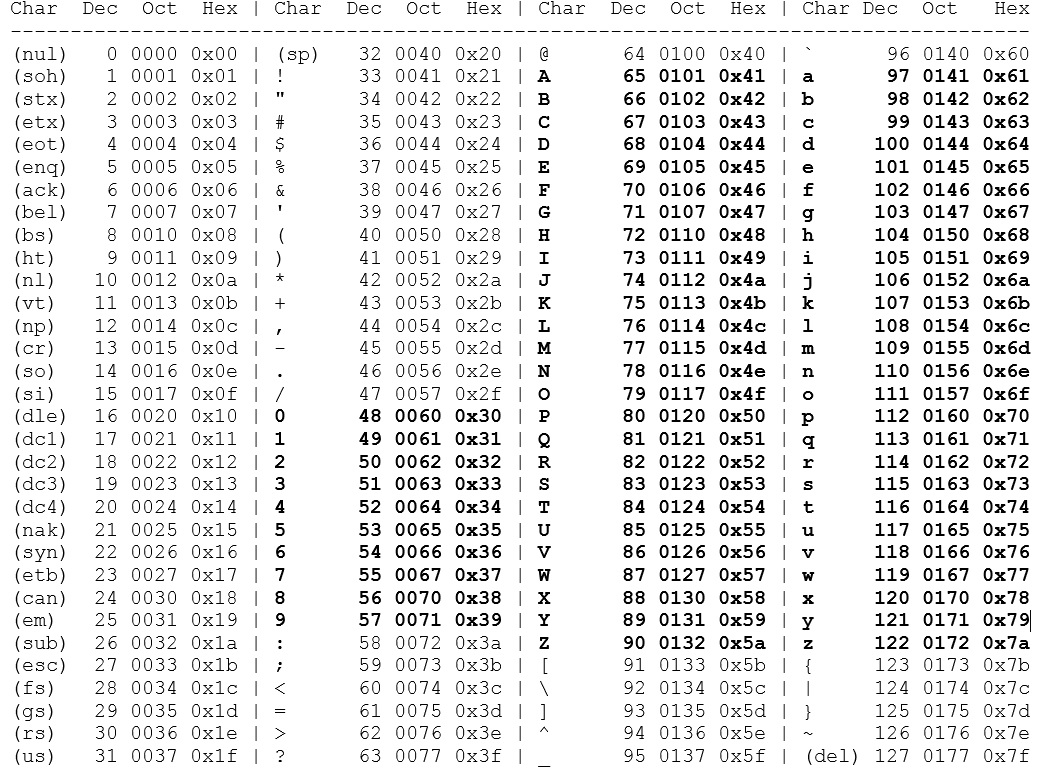
\includegraphics[width=0.68125\textwidth]{ascii.jpg}
\end{figure}

\newpage

\section{Primos até 10.000}

Existem 1.229 números primos até 10.000.

\begin{table}[h!]
\centering{
\begin{tabular}{|c|c|c|c|c|c|c|c|c|c|c|}
\hline
$2   $ & $3   $ & $5   $ & $7   $ & $11  $ & $13  $ & $17  $ & $19  $ & $23  $ & $29  $ & $31  $ \\
$37  $ & $41  $ & $43  $ & $47  $ & $53  $ & $59  $ & $61  $ & $67  $ & $71  $ & $73  $ & $79  $ \\
$83  $ & $89  $ & $97  $ & $101 $ & $103 $ & $107 $ & $109 $ & $113 $ & $127 $ & $131 $ & $137 $ \\
$139 $ & $149 $ & $151 $ & $157 $ & $163 $ & $167 $ & $173 $ & $179 $ & $181 $ & $191 $ & $193 $ \\
$197 $ & $199 $ & $211 $ & $223 $ & $227 $ & $229 $ & $233 $ & $239 $ & $241 $ & $251 $ & $257 $ \\
$263 $ & $269 $ & $271 $ & $277 $ & $281 $ & $283 $ & $293 $ & $307 $ & $311 $ & $313 $ & $317 $ \\
$331 $ & $337 $ & $347 $ & $349 $ & $353 $ & $359 $ & $367 $ & $373 $ & $379 $ & $383 $ & $389 $ \\
$397 $ & $401 $ & $409 $ & $419 $ & $421 $ & $431 $ & $433 $ & $439 $ & $443 $ & $449 $ & $457 $ \\
$461 $ & $463 $ & $467 $ & $479 $ & $487 $ & $491 $ & $499 $ & $503 $ & $509 $ & $521 $ & $523 $ \\
$541 $ & $547 $ & $557 $ & $563 $ & $569 $ & $571 $ & $577 $ & $587 $ & $593 $ & $599 $ & $601 $ \\
$607 $ & $613 $ & $617 $ & $619 $ & $631 $ & $641 $ & $643 $ & $647 $ & $653 $ & $659 $ & $661 $ \\
$673 $ & $677 $ & $683 $ & $691 $ & $701 $ & $709 $ & $719 $ & $727 $ & $733 $ & $739 $ & $743 $ \\
$751 $ & $757 $ & $761 $ & $769 $ & $773 $ & $787 $ & $797 $ & $809 $ & $811 $ & $821 $ & $823 $ \\
$827 $ & $829 $ & $839 $ & $853 $ & $857 $ & $859 $ & $863 $ & $877 $ & $881 $ & $883 $ & $887 $ \\
$907 $ & $911 $ & $919 $ & $929 $ & $937 $ & $941 $ & $947 $ & $953 $ & $967 $ & $971 $ & $977 $ \\
$983 $ & $991 $ & $997 $ & $1009$ & $1013$ & $1019$ & $1021$ & $1031$ & $1033$ & $1039$ & $1049$ \\
$1051$ & $1061$ & $1063$ & $1069$ & $1087$ & $1091$ & $1093$ & $1097$ & $1103$ & $1109$ & $1117$ \\
$1123$ & $1129$ & $1151$ & $1153$ & $1163$ & $1171$ & $1181$ & $1187$ & $1193$ & $1201$ & $1213$ \\
$1217$ & $1223$ & $1229$ & $1231$ & $1237$ & $1249$ & $1259$ & $1277$ & $1279$ & $1283$ & $1289$ \\
$1291$ & $1297$ & $1301$ & $1303$ & $1307$ & $1319$ & $1321$ & $1327$ & $1361$ & $1367$ & $1373$ \\
$1381$ & $1399$ & $1409$ & $1423$ & $1427$ & $1429$ & $1433$ & $1439$ & $1447$ & $1451$ & $1453$ \\
$1459$ & $1471$ & $1481$ & $1483$ & $1487$ & $1489$ & $1493$ & $1499$ & $1511$ & $1523$ & $1531$ \\
$1543$ & $1549$ & $1553$ & $1559$ & $1567$ & $1571$ & $1579$ & $1583$ & $1597$ & $1601$ & $1607$ \\
$1609$ & $1613$ & $1619$ & $1621$ & $1627$ & $1637$ & $1657$ & $1663$ & $1667$ & $1669$ & $1693$ \\
$1697$ & $1699$ & $1709$ & $1721$ & $1723$ & $1733$ & $1741$ & $1747$ & $1753$ & $1759$ & $1777$ \\
$1783$ & $1787$ & $1789$ & $1801$ & $1811$ & $1823$ & $1831$ & $1847$ & $1861$ & $1867$ & $1871$ \\
$1873$ & $1877$ & $1879$ & $1889$ & $1901$ & $1907$ & $1913$ & $1931$ & $1933$ & $1949$ & $1951$ \\
$1973$ & $1979$ & $1987$ & $1993$ & $1997$ & $1999$ & $2003$ & $2011$ & $2017$ & $2027$ & $2029$ \\
$2039$ & $2053$ & $2063$ & $2069$ & $2081$ & $2083$ & $2087$ & $2089$ & $2099$ & $2111$ & $2113$ \\
$2129$ & $2131$ & $2137$ & $2141$ & $2143$ & $2153$ & $2161$ & $2179$ & $2203$ & $2207$ & $2213$ \\
$2221$ & $2237$ & $2239$ & $2243$ & $2251$ & $2267$ & $2269$ & $2273$ & $2281$ & $2287$ & $2293$ \\
$2297$ & $2309$ & $2311$ & $2333$ & $2339$ & $2341$ & $2347$ & $2351$ & $2357$ & $2371$ & $2377$ \\
$2381$ & $2383$ & $2389$ & $2393$ & $2399$ & $2411$ & $2417$ & $2423$ & $2437$ & $2441$ & $2447$ \\
$2459$ & $2467$ & $2473$ & $2477$ & $2503$ & $2521$ & $2531$ & $2539$ & $2543$ & $2549$ & $2551$ \\
$2557$ & $2579$ & $2591$ & $2593$ & $2609$ & $2617$ & $2621$ & $2633$ & $2647$ & $2657$ & $2659$ \\
$2663$ & $2671$ & $2677$ & $2683$ & $2687$ & $2689$ & $2693$ & $2699$ & $2707$ & $2711$ & $2713$ \\
$2719$ & $2729$ & $2731$ & $2741$ & $2749$ & $2753$ & $2767$ & $2777$ & $2789$ & $2791$ & $2797$ \\
$2801$ & $2803$ & $2819$ & $2833$ & $2837$ & $2843$ & $2851$ & $2857$ & $2861$ & $2879$ & $2887$ \\
$2897$ & $2903$ & $2909$ & $2917$ & $2927$ & $2939$ & $2953$ & $2957$ & $2963$ & $2969$ & $2971$ \\
$2999$ & $3001$ & $3011$ & $3019$ & $3023$ & $3037$ & $3041$ & $3049$ & $3061$ & $3067$ & $3079$ \\
$3083$ & $3089$ & $3109$ & $3119$ & $3121$ & $3137$ & $3163$ & $3167$ & $3169$ & $3181$ & $3187$ \\
$3191$ & $3203$ & $3209$ & $3217$ & $3221$ & $3229$ & $3251$ & $3253$ & $3257$ & $3259$ & $3271$ \\
$3299$ & $3301$ & $3307$ & $3313$ & $3319$ & $3323$ & $3329$ & $3331$ & $3343$ & $3347$ & $3359$ \\
$3361$ & $3371$ & $3373$ & $3389$ & $3391$ & $3407$ & $3413$ & $3433$ & $3449$ & $3457$ & $3461$ \\
$3463$ & $3467$ & $3469$ & $3491$ & $3499$ & $3511$ & $3517$ & $3527$ & $3529$ & $3533$ & $3539$ \\
$3541$ & $3547$ & $3557$ & $3559$ & $3571$ & $3581$ & $3583$ & $3593$ & $3607$ & $3613$ & $3617$ \\
$3623$ & $3631$ & $3637$ & $3643$ & $3659$ & $3671$ & $3673$ & $3677$ & $3691$ & $3697$ & $3701$ \\
$3709$ & $3719$ & $3727$ & $3733$ & $3739$ & $3761$ & $3767$ & $3769$ & $3779$ & $3793$ & $3797$ \\
$3803$ & $3821$ & $3823$ & $3833$ & $3847$ & $3851$ & $3853$ & $3863$ & $3877$ & $3881$ & $3889$ \\
$3907$ & $3911$ & $3917$ & $3919$ & $3923$ & $3929$ & $3931$ & $3943$ & $3947$ & $3967$ & $3989$ \\
$4001$ & $4003$ & $4007$ & $4013$ & $4019$ & $4021$ & $4027$ & $4049$ & $4051$ & $4057$ & $4073$ \\
$4079$ & $4091$ & $4093$ & $4099$ & $4111$ & $4127$ & $4129$ & $4133$ & $4139$ & $4153$ & $4157$ \\
\hline
\end{tabular}
}
\end{table}

\begin{table}[h!]
\centering{
\begin{tabular}{|c|c|c|c|c|c|c|c|c|c|c|}
\hline
$4159$ & $4177$ & $4201$ & $4211$ & $4217$ & $4219$ & $4229$ & $4231$ & $4241$ & $4243$ & $4253$ \\
$4259$ & $4261$ & $4271$ & $4273$ & $4283$ & $4289$ & $4297$ & $4327$ & $4337$ & $4339$ & $4349$ \\
$4357$ & $4363$ & $4373$ & $4391$ & $4397$ & $4409$ & $4421$ & $4423$ & $4441$ & $4447$ & $4451$ \\
$4457$ & $4463$ & $4481$ & $4483$ & $4493$ & $4507$ & $4513$ & $4517$ & $4519$ & $4523$ & $4547$ \\
$4549$ & $4561$ & $4567$ & $4583$ & $4591$ & $4597$ & $4603$ & $4621$ & $4637$ & $4639$ & $4643$ \\
$4649$ & $4651$ & $4657$ & $4663$ & $4673$ & $4679$ & $4691$ & $4703$ & $4721$ & $4723$ & $4729$ \\
$4733$ & $4751$ & $4759$ & $4783$ & $4787$ & $4789$ & $4793$ & $4799$ & $4801$ & $4813$ & $4817$ \\
$4831$ & $4861$ & $4871$ & $4877$ & $4889$ & $4903$ & $4909$ & $4919$ & $4931$ & $4933$ & $4937$ \\
$4943$ & $4951$ & $4957$ & $4967$ & $4969$ & $4973$ & $4987$ & $4993$ & $4999$ & $5003$ & $5009$ \\
$5011$ & $5021$ & $5023$ & $5039$ & $5051$ & $5059$ & $5077$ & $5081$ & $5087$ & $5099$ & $5101$ \\
$5107$ & $5113$ & $5119$ & $5147$ & $5153$ & $5167$ & $5171$ & $5179$ & $5189$ & $5197$ & $5209$ \\
$5227$ & $5231$ & $5233$ & $5237$ & $5261$ & $5273$ & $5279$ & $5281$ & $5297$ & $5303$ & $5309$ \\
$5323$ & $5333$ & $5347$ & $5351$ & $5381$ & $5387$ & $5393$ & $5399$ & $5407$ & $5413$ & $5417$ \\
$5419$ & $5431$ & $5437$ & $5441$ & $5443$ & $5449$ & $5471$ & $5477$ & $5479$ & $5483$ & $5501$ \\
$5503$ & $5507$ & $5519$ & $5521$ & $5527$ & $5531$ & $5557$ & $5563$ & $5569$ & $5573$ & $5581$ \\
$5591$ & $5623$ & $5639$ & $5641$ & $5647$ & $5651$ & $5653$ & $5657$ & $5659$ & $5669$ & $5683$ \\
$5689$ & $5693$ & $5701$ & $5711$ & $5717$ & $5737$ & $5741$ & $5743$ & $5749$ & $5779$ & $5783$ \\
$5791$ & $5801$ & $5807$ & $5813$ & $5821$ & $5827$ & $5839$ & $5843$ & $5849$ & $5851$ & $5857$ \\
$5861$ & $5867$ & $5869$ & $5879$ & $5881$ & $5897$ & $5903$ & $5923$ & $5927$ & $5939$ & $5953$ \\
$5981$ & $5987$ & $6007$ & $6011$ & $6029$ & $6037$ & $6043$ & $6047$ & $6053$ & $6067$ & $6073$ \\
$6079$ & $6089$ & $6091$ & $6101$ & $6113$ & $6121$ & $6131$ & $6133$ & $6143$ & $6151$ & $6163$ \\
$6173$ & $6197$ & $6199$ & $6203$ & $6211$ & $6217$ & $6221$ & $6229$ & $6247$ & $6257$ & $6263$ \\
$6269$ & $6271$ & $6277$ & $6287$ & $6299$ & $6301$ & $6311$ & $6317$ & $6323$ & $6329$ & $6337$ \\
$6343$ & $6353$ & $6359$ & $6361$ & $6367$ & $6373$ & $6379$ & $6389$ & $6397$ & $6421$ & $6427$ \\
$6449$ & $6451$ & $6469$ & $6473$ & $6481$ & $6491$ & $6521$ & $6529$ & $6547$ & $6551$ & $6553$ \\
$6563$ & $6569$ & $6571$ & $6577$ & $6581$ & $6599$ & $6607$ & $6619$ & $6637$ & $6653$ & $6659$ \\
$6661$ & $6673$ & $6679$ & $6689$ & $6691$ & $6701$ & $6703$ & $6709$ & $6719$ & $6733$ & $6737$ \\
$6761$ & $6763$ & $6779$ & $6781$ & $6791$ & $6793$ & $6803$ & $6823$ & $6827$ & $6829$ & $6833$ \\
$6841$ & $6857$ & $6863$ & $6869$ & $6871$ & $6883$ & $6899$ & $6907$ & $6911$ & $6917$ & $6947$ \\
$6949$ & $6959$ & $6961$ & $6967$ & $6971$ & $6977$ & $6983$ & $6991$ & $6997$ & $7001$ & $7013$ \\
$7019$ & $7027$ & $7039$ & $7043$ & $7057$ & $7069$ & $7079$ & $7103$ & $7109$ & $7121$ & $7127$ \\
$7129$ & $7151$ & $7159$ & $7177$ & $7187$ & $7193$ & $7207$ & $7211$ & $7213$ & $7219$ & $7229$ \\
$7237$ & $7243$ & $7247$ & $7253$ & $7283$ & $7297$ & $7307$ & $7309$ & $7321$ & $7331$ & $7333$ \\
$7349$ & $7351$ & $7369$ & $7393$ & $7411$ & $7417$ & $7433$ & $7451$ & $7457$ & $7459$ & $7477$ \\
$7481$ & $7487$ & $7489$ & $7499$ & $7507$ & $7517$ & $7523$ & $7529$ & $7537$ & $7541$ & $7547$ \\
$7549$ & $7559$ & $7561$ & $7573$ & $7577$ & $7583$ & $7589$ & $7591$ & $7603$ & $7607$ & $7621$ \\
$7639$ & $7643$ & $7649$ & $7669$ & $7673$ & $7681$ & $7687$ & $7691$ & $7699$ & $7703$ & $7717$ \\
$7723$ & $7727$ & $7741$ & $7753$ & $7757$ & $7759$ & $7789$ & $7793$ & $7817$ & $7823$ & $7829$ \\
$7841$ & $7853$ & $7867$ & $7873$ & $7877$ & $7879$ & $7883$ & $7901$ & $7907$ & $7919$ & $7927$ \\
$7933$ & $7937$ & $7949$ & $7951$ & $7963$ & $7993$ & $8009$ & $8011$ & $8017$ & $8039$ & $8053$ \\
$8059$ & $8069$ & $8081$ & $8087$ & $8089$ & $8093$ & $8101$ & $8111$ & $8117$ & $8123$ & $8147$ \\
$8161$ & $8167$ & $8171$ & $8179$ & $8191$ & $8209$ & $8219$ & $8221$ & $8231$ & $8233$ & $8237$ \\
$8243$ & $8263$ & $8269$ & $8273$ & $8287$ & $8291$ & $8293$ & $8297$ & $8311$ & $8317$ & $8329$ \\
$8353$ & $8363$ & $8369$ & $8377$ & $8387$ & $8389$ & $8419$ & $8423$ & $8429$ & $8431$ & $8443$ \\
$8447$ & $8461$ & $8467$ & $8501$ & $8513$ & $8521$ & $8527$ & $8537$ & $8539$ & $8543$ & $8563$ \\
$8573$ & $8581$ & $8597$ & $8599$ & $8609$ & $8623$ & $8627$ & $8629$ & $8641$ & $8647$ & $8663$ \\
$8669$ & $8677$ & $8681$ & $8689$ & $8693$ & $8699$ & $8707$ & $8713$ & $8719$ & $8731$ & $8737$ \\
$8741$ & $8747$ & $8753$ & $8761$ & $8779$ & $8783$ & $8803$ & $8807$ & $8819$ & $8821$ & $8831$ \\
$8837$ & $8839$ & $8849$ & $8861$ & $8863$ & $8867$ & $8887$ & $8893$ & $8923$ & $8929$ & $8933$ \\
$8941$ & $8951$ & $8963$ & $8969$ & $8971$ & $8999$ & $9001$ & $9007$ & $9011$ & $9013$ & $9029$ \\
$9041$ & $9043$ & $9049$ & $9059$ & $9067$ & $9091$ & $9103$ & $9109$ & $9127$ & $9133$ & $9137$ \\
$9151$ & $9157$ & $9161$ & $9173$ & $9181$ & $9187$ & $9199$ & $9203$ & $9209$ & $9221$ & $9227$ \\
$9239$ & $9241$ & $9257$ & $9277$ & $9281$ & $9283$ & $9293$ & $9311$ & $9319$ & $9323$ & $9337$ \\
$9341$ & $9343$ & $9349$ & $9371$ & $9377$ & $9391$ & $9397$ & $9403$ & $9413$ & $9419$ & $9421$ \\
$9431$ & $9433$ & $9437$ & $9439$ & $9461$ & $9463$ & $9467$ & $9473$ & $9479$ & $9491$ & $9497$ \\
$9511$ & $9521$ & $9533$ & $9539$ & $9547$ & $9551$ & $9587$ & $9601$ & $9613$ & $9619$ & $9623$ \\
$9629$ & $9631$ & $9643$ & $9649$ & $9661$ & $9677$ & $9679$ & $9689$ & $9697$ & $9719$ & $9721$ \\
$9733$ & $9739$ & $9743$ & $9749$ & $9767$ & $9769$ & $9781$ & $9787$ & $9791$ & $9803$ & $9811$ \\
$9817$ & $9829$ & $9833$ & $9839$ & $9851$ & $9857$ & $9859$ & $9871$ & $9883$ & $9887$ & $9901$ \\
$9907$ & $9923$ & $9929$ & $9931$ & $9941$ & $9949$ & $9967$ & $9973$ &        &        &       \\
\hline

\end{tabular}
}
\end{table}